\documentclass{article}

%% doc settings
\hyphenchar\font=-1 % suppress hyphenation
\setlength\parindent{0pt} % suppress indentation
\usepackage[margin=1.25truein]{geometry} % set page margins

%% libraries 
\usepackage{listings}
\usepackage{fancyhdr}
\usepackage{lastpage}
\usepackage{url}
\usepackage{xcolor}
\usepackage{hyperref}
\usepackage{amssymb}
\usepackage{amsthm}
\usepackage{amsmath}
\usepackage{natbib}
\usepackage{tikz}
\usepackage{pgfplots}
\usepackage{textcomp}
\usepackage{subcaption}
\usetikzlibrary{shapes, arrows}

%% link viz
\hypersetup{
    colorlinks = true,
    linkcolor = red,
    urlcolor = red,
    citecolor = black
}

%% code colors 
\definecolor{codegreen}{rgb}{0,0.6,0}
\definecolor{codegray}{rgb}{0.5,0.5,0.5}
\definecolor{codepurple}{rgb}{0.58,0,0.82}
\definecolor{backcolour}{rgb}{0.95,0.95,0.92}

\lstdefinestyle{mystyle}{
    backgroundcolor=\color{backcolour},   
    commentstyle=\color{codegreen},
    keywordstyle=\color{magenta},
    numberstyle=\tiny\color{codegray},
    stringstyle=\color{codepurple},
    basicstyle=\ttfamily\footnotesize,
    breakatwhitespace=false,         
    breaklines=true,                 
    captionpos=b,                    
    keepspaces=true,                 
    numbers=left,                    
    numbersep=5pt,                  
    showspaces=false,                
    showstringspaces=false,
    showtabs=false,                  
    tabsize=2
}

\lstset{style=mystyle}

%% page nums
\pagestyle{fancy}
\fancyhf{}
\fancyfoot[C]{Pg. \thepage \space of \pageref*{LastPage}}
\renewcommand{\headrulewidth}{0pt}

%% begin doc
\begin{document}
\title{SYSEN 6000: Foundations of Complex Systems\\~\\
    \Large Deterministic Global Optimization
}
\author{
    Nick Kunz [NetID: \url{nhk37}] \hyperlink{nhk37@cornell.edu}{nhk37@cornell.edu}}
\date{October 31, 2022}
\maketitle
\thispagestyle{fancy}

%% body doc
\section*{Integer Programming}
Given that:
\begin{equation}
\begin{split}
    \text{max \space} & y_1 + 1.2y_2\\
    \text{s.t. \space} & \space y_1 + y_2 \leq 1\\
    & 0.8y_1 + 1.1y_2 \leq 1\\
    & y_1, y_2 = \{0, 1\}
\end{split}
\end{equation}

When the binary variables are relaxed to continuous ones, such that $y_1, y_2 \in [0, 1]$, the contours of the objective and the feasible region can be exhibited as:

    \begin{center}
        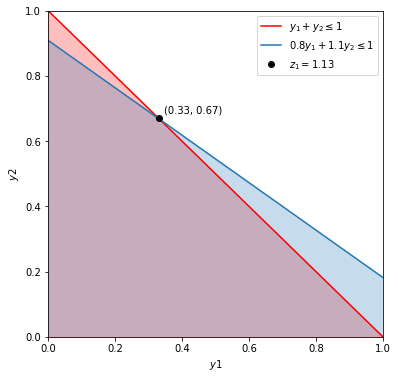
\includegraphics[width=0.50\textwidth]{zeee.png}
    \end{center}

From inspection, the optimal solution to the relaxed problem, such that $y_1, y_2 \in [0, 1]$, is:

    \begin{equation}
        y_1 = \frac{1}{3}, y_2 = \frac{2}{3}\\~\\
    \end{equation}
    \begin{equation}\nonumber
        z_1 = 1.13
    \end{equation}

Enumerating all $y_1, y_2$ integer combinations $[0,1]$ the solution space can be expressed as:
    \begin{equation}\nonumber
        y_1 = 0, y_2 = 0
    \end{equation}
    \begin{equation}
        y_1 = 0, y_2 = 1
    \end{equation}
    \begin{equation}\nonumber
        y_1 = 1, y_2 = 1
    \end{equation}
    \begin{equation}\nonumber
        y_1 = 1, y_2 = 0
    \end{equation}

    which can be exhibited as:
    \begin{center}
        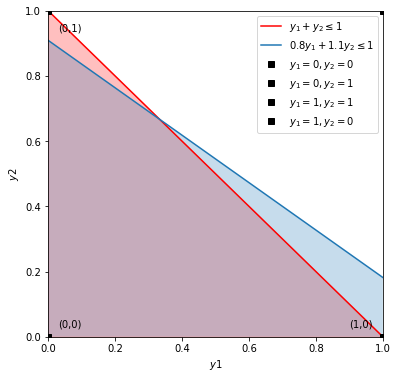
\includegraphics[width=0.50\textwidth]{comb.png}
    \end{center}

Therefore, the optimal solution is:

    \begin{equation}
        y_1 = 1, y_2 = 0
    \end{equation}\\

    \item The branch and bound method for solving LP subproblems can be exhibited as:

    \begin{figure}[h]
    \centering
    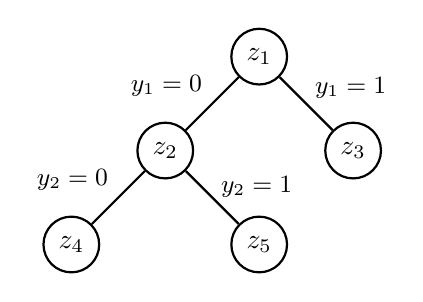
\begin{tikzpicture}[-,>=stealth',auto,node distance=48pt,
      thick,main node/.style={circle,,draw}, other node/.style={}]
    
        \node[main node] (1) {$z_1$};
        \node[main node] (2) [below left of=1] {$z_2$};
        \node[main node] (3) [below right of=1] {$z_3$};
        \node[main node] (4) [below left of=2] {$z_4$};
        \node[main node] (5) [below right of=2] {$z_5$};
        
        \path[every node/.style={font=\sffamily\small}]
            (1) edge node [xshift=0pt, yshift=10pt, label=left:{$y_1=0$}]{} (2)
            (1) edge node [xshift=-8pt, yshift=2pt, label=right:{$y_1=1$}]{} (3)
            (2) edge node [xshift=0pt, yshift=10pt, label=left:{$y_2=0$}]{} (4)
            (2) edge node [xshift=-8pt, yshift=0pt, label=right:{$y_2=1$}]{} (5)
        ;
    \end{tikzpicture}
    \end{figure}

where: 
\begin{equation}
\begin{split}
    z_1 & = 1.13\\
    z_2 & = 1.091\\
    z_3 & = 1\\
    z_4 & = 0\\
    z_5 & = \cdot 
\end{split}
\end{equation}

Therefore, the optimal solution is:
\begin{equation}
    y_1 = 1, y_2 = 0\\
\end{equation}
\begin{equation}\nonumber
    z_3 = 1
\end{equation}


\section*{Gomory Cut}
Given the inequality: 
\begin{equation}
\begin{split}
    y_2 + y_3 + 2y_4 \leq 6
\end{split}
\end{equation}

and the region:
\begin{equation}
    X = \{y \in Z_4: 4y_1 + 5y_2 + 9y_3 + 12y_4 \leq 34 \}
\end{equation}

It is provably valid by:
\begin{equation}
\begin{split}
    \frac{4}{5} y_1 + \frac{5}{5}y_2 + \frac{9}{5}y_3 + \frac{12}{5}y_4 \leq \frac{34}{5} \Longrightarrow 0\frac{4}{5} y_1 + y_2 + 1\frac{4}{5}y_3 + 2\frac{2}{5}y_4 \leq \frac{34}{5}\\
\end{split}
\end{equation}

when considering:
\begin{equation}
\begin{split}
    \sum_{j} a_{ij}^{*}y_j \leq b_i, y_j \in \{0, 1\}
\end{split}
\end{equation}

which is given by:
\begin{equation}
\begin{split}
    \sum_{j} \lfloor{a_{ij}}\rfloor y_j \leq \lfloor{b_i}\rfloor
\end{split}
\end{equation}

and when applied is:
\begin{equation}
\begin{split}
    0 \cdot y_1 + y_2 + 1 \cdot y_3 + 2 \cdot y_4 \leq 6
\end{split}
\end{equation}

which results in the given inequality:
\begin{equation}
\begin{split}
    y_2 + y_3 + 2y_4 \leq 6
\end{split}
\end{equation}

\section*{Mixed-Integer Non-Linear Programming}
Given that:
\begin{equation}
\begin{split}
    \text{min \space} & f = y_1 + 1.5y_2 + 0.5y_3 + x_{1}^{2} + x_{2}^{2}\\
    \text{s.t. \space} 
    & \space (x_1 - 2)^2 -x_2 \leq 0\\
    & x_1 - 2y_1 \geq 0\\
    & x_1 - x_2 - 4(1-y_1) \leq 0\\
    & x_1 - (1 - y_1) \geq 0\\
    & x_2 - y_2 \geq 0\\
    & x_1 + x_2 \geq 3y_3\\
    & y_1 + y_2 + y_3 \geq 1\\
    & 0 \leq x_1 \leq 4, 0 \leq x_2 \leq 4\\
    & y_1, y_2, y_3 = \{0, 1\}\\
\end{split}
\end{equation}

the inequalities can be reformulated as:
\begin{equation}
\begin{split}
    \text{s.t. \space} 
    & \space (x_1 - 2)^2 -x_2 \leq 0\\
    & -(x_1 - 2y_1) \leq 0\\
    & x_1 - x_2 - 4(1-y_1) \leq 0\\
    & - x_1 - (1 - y_1) \leq 0\\
    & - (x_2 + y_2) \leq 0\\
    & - (x_2 + y_2 - 3y_3)\leq 0\\
    & - (y_1 + y_2 + y_3 - 1) \leq 0
\end{split}
\end{equation}

Let $y_1 = y_2 = y_3 = 1$, so that:
\begin{equation}
\begin{split}
    \text{min \space} & f = 3 + x_{1}^{2} + x_{2}^{2}\\
    \text{s.t. \space} 
    & \space (x_1 - 2)^2 -x_2 \leq 0\\
    & -(x_1 - 2 \cdot 1) \leq 0\\
    & x_1 - x_2 - 4(1 - 1) \leq 0\\
    & - x_1 - (1 - 1) \leq 0\\
    & - (x_2 + 1) \leq 0\\
    & - (x_2 + 1 - 3 \cdot 1)\leq 0\\
    & - (1 + 1 + 1 - 1) \leq 0\\
    & 0 \leq x_1 \leq 4, 0 \leq x_2 \leq 4\\
    & y_1, y_2, y_3 = \{0, 1\}\\
\end{split}
\end{equation}
\\
which results in $x_{1}^{*} = 2, x_{2}^{*} = 2, UB_1 = 5$, where we can continue to solve for:
\begin{equation}
\begin{split}
\nabla f & = 
    \begin{bmatrix}
        2 \cdot 2\\
        2 \cdot 2\\
    \end{bmatrix} \Longrightarrow
\nabla f^* = 
    \begin{bmatrix}
        4\\
        4\\
    \end{bmatrix}
\end{split}
\end{equation}
\begin{equation}
\begin{split}
    f_{Lin} 
        & = f(x^*) + \nabla f(x^*) + (x-x^*)\\
        & = 8 + 
            \begin{bmatrix}
                4\\
                4\\
            \end{bmatrix}
            \begin{bmatrix}
                2 - 2\\
                2 - 2\\
            \end{bmatrix}\\
        & = 8 + 4(2 - 2) + 4(2 - 2) + \\
        & \text{\space\space\space} (y_1 + 1.5y_2 + 0.5y_3)
\end{split}
\end{equation}

\begin{equation}
\begin{split}
\nabla g & = 
    \begin{bmatrix}
        2(2 - 2)\\
        -1\\
    \end{bmatrix} \Longrightarrow
\nabla g^* = 
    \begin{bmatrix}
        0\\
        -1\\
    \end{bmatrix}
\end{split}
\end{equation}
\begin{equation}
\begin{split}
    g_{Lin} 
        & = g(x^*) + \nabla g(x^*) + (x-x^*)\\
        & = -2 + 
            \begin{bmatrix}
                0\\
                -1\\
            \end{bmatrix}
            \begin{bmatrix}
                2 - 2\\
                2 - 2\\
            \end{bmatrix}\\
        & = -2 - (2 - 2) \leq 0
\end{split}
\end{equation}
\\~\\
Hence $x_{1}^{*} = 1, x_{2}^{*} = 1, y_1 = 0, y_2 = 1, y_3 = 0, LB_1 = 3.5$, when min $\alpha$, s.t. $\alpha \geq f_Lin, g_Lin \leq 0$, and the reformulated constraints, where the $UB_1 > LB_1$.\\

Now let $y_1 = 0, y_2 = 1, y_3 = 0$, so that:
\begin{equation}
\begin{split}
    \text{min \space} & f = 1.5 + x_{1}^{2} + x_{2}^{2}\\
    \text{s.t. \space} 
    & \space (x_1 - 2)^2 -x_2 \leq 0\\
    & - x_1 \leq 0\\
    & x_1 - x_2 - 4 \leq 0\\
    & - x_1 - 1 \leq 0\\
    & - x_2 + 1 \leq 0\\
    & - x_1 - x_2 \leq 0\\
    & - x_2 \leq 0\\
    & x_1 - 4 \leq 0\\
    & x_2 - 4 \leq 0\\
    & 0 \leq x_1 \leq 4, 0 \leq x_2 \leq 4\\
    & y_1, y_2, y_3 = \{0, 1\}\\
\end{split}
\end{equation}\\

Hence $x_{1}^{*} = 1, x_{2}^{*} = 1, y_1 = 0, y_2 = 1, y_3 = 0, UB_2 = 3.5$, when min $\alpha$, s.t. $\alpha \geq f_Lin, g_Lin \leq 0$, and the reformulated constraints, where $UB_2 = LB_1$.\\

Here the stopping criteria $UB = LB$ has been satisfied, where the optimal solution is:
    \begin{equation}\nonumber
        x_1 = 1, x_2 = 1\\
    \end{equation}
    \begin{equation}
        y_1 = 0, y_2 = 1, y_3 = 0\\
    \end{equation}
    \begin{equation}\nonumber
        z_3 = 3.5
    \end{equation}
\\~\\
\section*{Mixed-Integer Linear Fractional Programming}
Given that:
    \begin{equation}
    \begin{split}
        \text{max \space} & \frac{2x + 4y_1 + 3y_2}{x + y_1 + 1}\\
        \text{s.t. \space} & \space 4x - y_1 - 4y_2 \leq 1\\
        & 5x + 4y_1 + 2y_2 \leq 3\\
        & x \geq 0\\
        & y_1, y_2 \in \{0, 1\}
    \end{split}
    \end{equation}
\\~\\
The parametric algorithm applies $q$, which reformulates into:
    \begin{equation}
    \begin{split}
        \text{max\space} & (2x + 4y_1 + 3y_2) - q \cdot (x + y_1 + 1)\\
        \text{s.t. \space} & x + y_1 + 1 > 0\\
        & \space 4x - y_1 - 4y_2 \leq 1\\
        & 5x + 4y_1 + 2y_2 \leq 3\\
        & x \geq 0\\
        & y_1, y_2 \in \{0, 1\}
    \end{split}
    \end{equation}
\\~\\
that when solved, the optimal solution is:
    \begin{equation}\nonumber
        x = 0\\
    \end{equation}
    \begin{equation}
        y_1 = 0, y_2 = 1\\
    \end{equation}
\\~\\
The reformulation-linearization algorithm applies $g$ and $z$, which reformulates into:
    \begin{equation}
    \begin{split}
        \text{max\space} & 2 \cdot z + 4\cdot g \cdot y_1 + 3 \cdot g \cdot y_2 \\
        \text{s.t. \space} & z + g \cdot y_1 + 1 \cdot g = 1\\
        & \space 4 \cdot z - g \cdot y_1 - 4 \cdot g \cdot y_2 \leq 1\\
        & 5 \cdot z + 4 \cdot g \cdot y_1 + 2 \cdot g \cdot y_2 \leq 3\\
        & z \geq 0, g \geq 0\\
        & y_1, y_2 \in \{0, 1\}
    \end{split}
    \end{equation}

and with $w_1$ and $w_2$, further into: 
    \begin{equation}
    \begin{split}
        \text{max\space} & 2 \cdot z + 4 \cdot w_1 + 3 \cdot w_2\\
        \text{s.t. \space} & z + w_1 + 1 \cdot g = 1\\
        & \space 4 \cdot z - w_1 - 4 \cdot w_2 - g \leq 0\\
        & 5 \cdot z + 4 \cdot w_1 + 2 \cdot w_2 - 3 \cdot g \leq 0\\
        & 0 \leq w_1 \leq M \cdot y_1\\
        & 0 \leq w_2 \leq M \cdot y_2\\
        & w_1 \leq g\\
        & w_2 \leq g\\
        & w_1 \geq g - M(1 - y_1)\\
        & w_2 \geq g - M(1 - y_2)\\
        & z \geq 0\\
        & g \geq 0\\
        & w_1 \geq 0\\
        & w_2 \geq 0\\
        & y_1, y_2 \in \{0, 1\}
    \end{split}
    \end{equation}

where:
    \begin{equation}\nonumber
        z = g \cdot x
    \end{equation}
    \begin{equation}
        g = \frac{1}{x + y_1 + 1}
    \end{equation}
    \begin{equation}\nonumber
        w_1 = g \cdot y_1, w_2 = g \cdot y_2 
    \end{equation}
\\~\\
that when solved, the optimal solution is:
    \begin{equation}\nonumber
        z = 0        
    \end{equation}
    \begin{equation}\nonumber
        g = 1
    \end{equation}
    \begin{equation}
        w_1 = 0, w_2 = 1
    \end{equation}
    \begin{equation}\nonumber
        y_1 = 0, y_2 = 1
    \end{equation}

\newpage
\section*{Appendix}
\begin{enumerate}
    \item Integer Programming
    \begin{lstlisting}[language=Python, title=Python 3: Integer Programming Solution to the Relaxed Problem]
## librarires
import numpy as np
from scipy.optimize import linprog
import matplotlib.pyplot as plt

## minimize objective 
## (inversed original maximize)
obj = [-1.0, -1.2]

## constraints
## left side inequalities
lft_ieq = [
    [1.0, 1.0],
    [0.8, 1.1]
]

## right side inequalities
rgt_ieq = [
    1.0,
    1.0
]

## global bounds
gbl_bds = [
    [0.0, 1.0], ## y1
    [0.0, 1.0] ## y2
]

## optimize
opt = linprog(
    c = obj,
    A_ub = lft_ieq, 
    b_ub = rgt_ieq,
    bounds = gbl_bds,
    method = 'simplex'
)

## solution
y1 = round(
    number = opt.x[0],
    ndigits = 2
)

y2 = round(
    number = opt.x[1],
    ndigits = 2
)

z = round(
    number = -opt.fun,
    ndigits = 2
)

print('y1 = {x}'.format(x = y1))
print('y2 = {x}'.format(x = y2))
print('z = {x}'.format(x = z))\end{lstlisting}

\newpage
\item Continuous Contours 
\begin{lstlisting}[language=Python, title=Python 3: Contours of the Relaxed Problem]
## librarires
import numpy as np
import matplotlib.pyplot as plt

## space
x = np.linspace(0, 1, 100)

## constraints
y1 = (1 - x)
y2 = (0.8 / -1.1) * x + (-1.0 / -1.1)

## plot
plt.figure(figsize=(6,6))
plt.plot(x, y1, 
    color = 'red', 
    label = r'$y_1 + y_2 \leq 1$'
)
plt.plot(
    x, y2, 
    label = r'$0.8y_1 + 1.1y_2 \leq 1$'
)

plt.plot(
    0.33, 0.67, 'o', 
    color = 'black', 
    label = r'$z_1 = 1.13$'
)

plt.annotate(
    s = '(0.33, 0.67)', 
    xy = (0.33, 0.67), 
    textcoords = "offset points", 
    xytext = (5, 5), 
    ha = 'left'
)

plt.fill_between(
    x, y1, 
    color = 'red', 
    alpha = 0.25
)

plt.fill_between(
    x, y2, 
    alpha = 0.25
)

plt.xlabel(r'$y1$')
plt.ylabel(r'$y2$')
plt.xlim(0, 1)
plt.ylim(0, 1)

plt.legend(
    bbox_to_anchor = (1, 1), 
    loc = 0, 
    borderaxespad = 0.5
)

plt.show()\end{lstlisting}

\newpage
\item Enumerated Combinations
\begin{lstlisting}[language=Python, title=Python 3: Enumerated Combinations for the Optimal Solution]
## librarires
import numpy as np
import matplotlib.pyplot as plt

## space
x = np.linspace(0, 1, 100)

## constraints
y1 = (1 - x)
y2 = (0.8 / -1.1) * x + (-1.0 / -1.1)

## plot
plt.figure(figsize=(6,6))
plt.plot(
    x, y1, 
    color = 'red', 
    label = r'$y_1 + y_2 \leq 1$'
)

plt.plot(
    x, y2, 
    label = r'$0.8y_1 + 1.1y_2 \leq 1$'
)

plt.plot(
    0, 0, 's', 
    color = 'black', 
    label = r'$y_1 = 0, y_2 = 0$'
)

plt.plot(
    0, 1, 's', 
    color = 'black', 
    label = r'$y_1 = 0, y_2 = 1$'
)

plt.plot(
    1, 1, 's', 
    color = 'black', 
    label = r'$y_1 = 1, y_2 = 1$'
)

plt.plot(
    1, 0, 's', 
    color = 'black', 
    label = r'$y_1 = 1, y_2 = 0$'
)

plt.annotate(
    s = '(0,0)', 
    xy = (0, 0), 
    textcoords = "offset points", 
    xytext = (10, 10), 
    ha = 'left'
)

plt.annotate(
    s = '(0,1)', 
    xy = (0, 1), 
    textcoords = "offset points", 
    xytext = (10, -20), 
    ha = 'left'
)

plt.annotate(
    s = '(1,0)', 
    xy = (1, 0), 
    textcoords = "offset points", 
    xytext = (-10, 10), 
    ha = 'right'
)

plt.fill_between(
    x, y1, 
    color = 'red', 
    alpha = 0.25
)

plt.fill_between(
    x, y2, 
    alpha = 0.25
)

plt.xlabel(r'$y1$')
plt.ylabel(r'$y2$')
plt.xlim(0, 1)
plt.ylim(0, 1)

plt.legend(
    bbox_to_anchor = (1, 1), 
    loc = 0,
    borderaxespad = 0.5
)

plt.show()

## happy halloween!\end{lstlisting}

\end{enumerate}
\end{document}